\chapter{Test}

\section{Base dei test}
Per testare l'effettivo funzionamento dell'applicazione ho usato alcune stanze di casa mia ed ho assegnato a ciascuna di esse una \textit{label}. Qui di seguito una piccola piantina rappresentante le stanze utilizzate:

\begin{figure}[H]
\centering
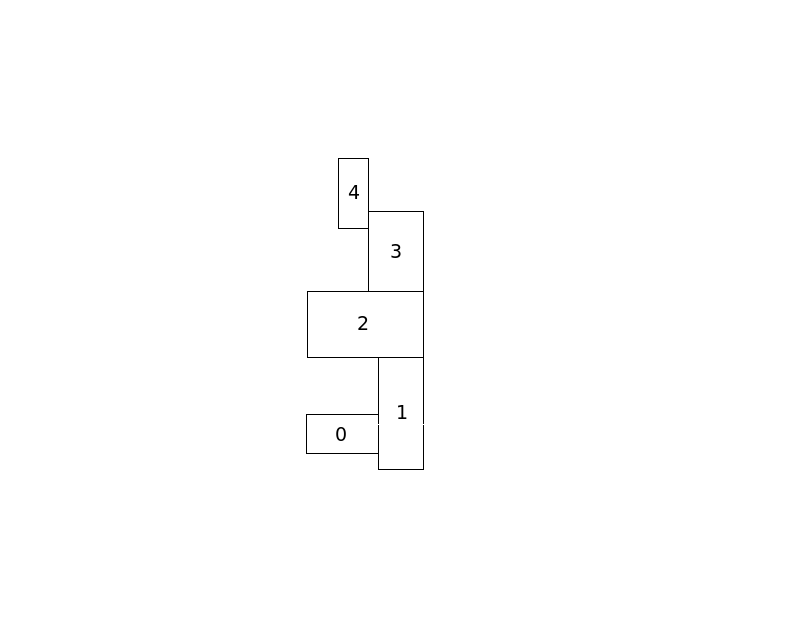
\includegraphics[width=0.7\linewidth]{img/test_pianta_casa}
\caption{Una piccola raffigurazione delle stanze usate per le prove con sopra scritto la \textit{label} assegnata}
\label{fig:test_pianta_casa}
\end{figure}

Sono stati raccolti circa 18000 campioni di onde magnetiche. La suddivisione fra addestramento e test e' 70/30.

\section{Caratteristiche}
Dai grafici qui di seguito possiamo notare che c'e' sovrapposizione fra i dati, quindi e' presente del rumore nei dati.
\begin{figure}[H]
	\centering
	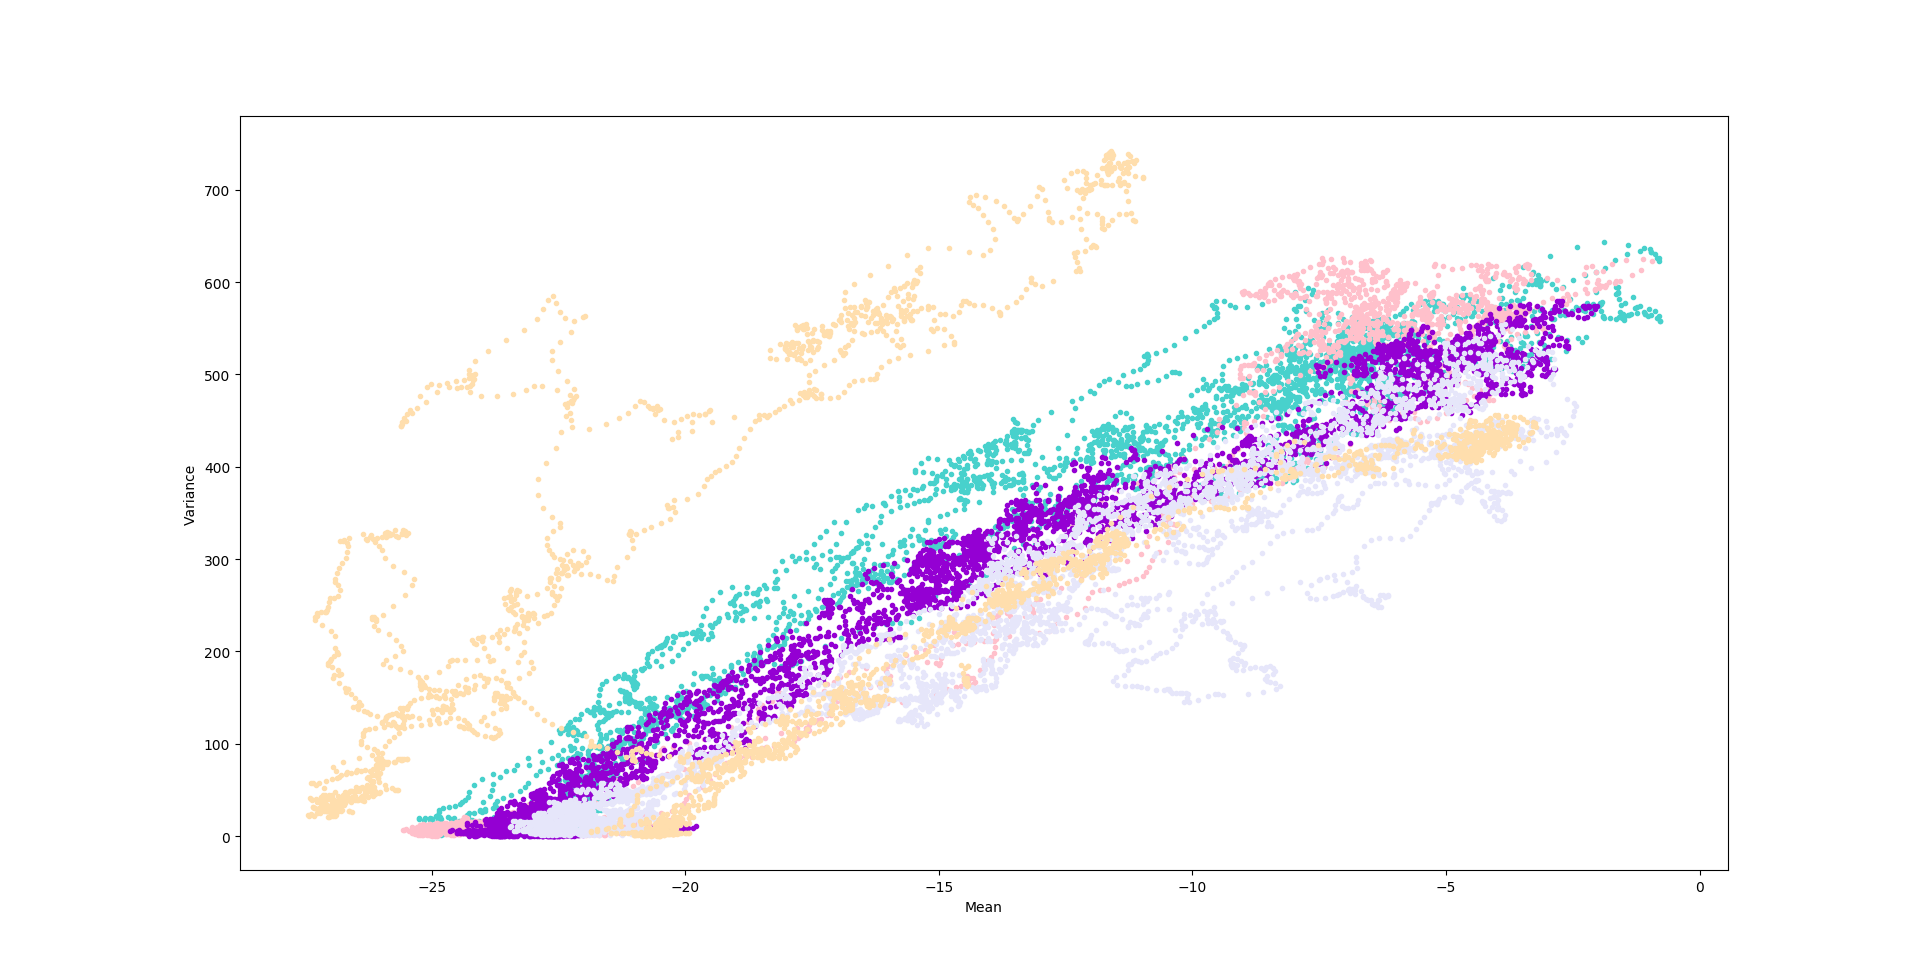
\includegraphics[width=1\linewidth]{img/plot_features}
	\caption{Grafico in 2 dimensioni della media e varianza di tutte le onde magnetiche. I colori dei punti rappresentano le etichette}
	\label{fig:plotfeatures}
\end{figure}

La causa del rumore sono i sensori che offrono una misurazione non precisa. Un possibile riparo al problema e' il \textit{filtro di Kalman}

\section{Classificatori a confronto}
Qui di seguito vediamo i risultati ottenuti da ciascun classificatore con un istogramma:

\begin{figure}[H]
	\centering
	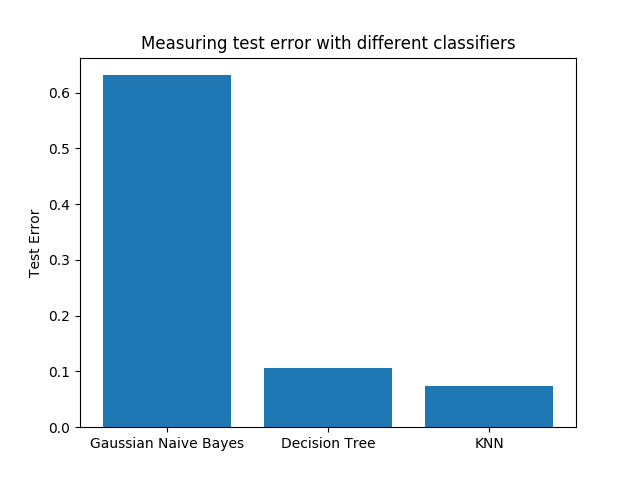
\includegraphics[width=0.7\linewidth]{img/test_errors}
	\caption{}
	\label{fig:testerrors}
\end{figure}

come possiamo notare \textit{Gaussian Naive Bayes} e' totalmente inadatto alla classificazione di onde magnetiche mentre gli alberi di decisione e \textit{K Nearest Neightbours} si comportano molto bene, con risultati leggermente migliori in quest'ultimo.
A questo punto qualcuno potrebbe pero' pensare che gli ultimi 2 modelli si sono sovradattati agli esempi (\textit{overfitting}) ed avrebbe ragione, perche' applicando la \textit{cross validation} abbiamo risultati diversi da quelli precedenti.

\begin{figure}[H]
	\centering
	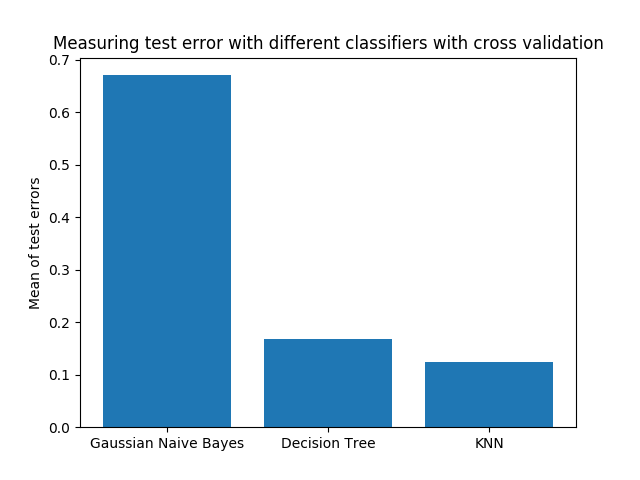
\includegraphics[width=0.7\linewidth]{img/test_errors_cross_validation}
	\caption{}
	\label{fig:testerrorscrossvalidation}
\end{figure}

Adesso visualizziamo gli errori per etichetta:

\begin{figure}[H]
	\centering
	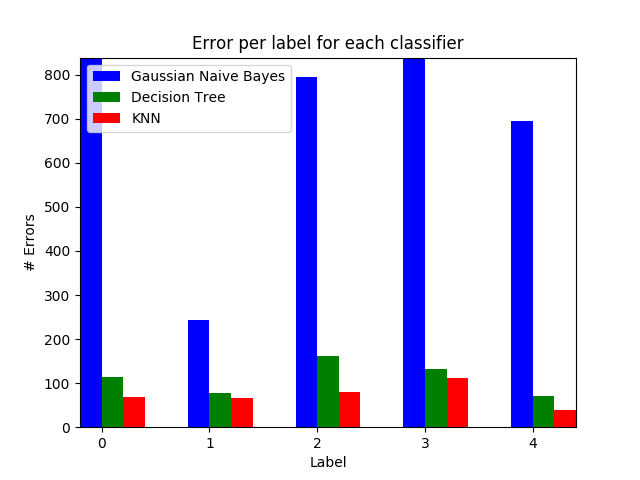
\includegraphics[width=0.7\linewidth]{img/test_error_per_label}
	\caption{Numero di errori nella predizione per etichetta}
	\label{fig:testerrorperlabel}
\end{figure}
\medskip
\begin{figure}[H]
	\centering
	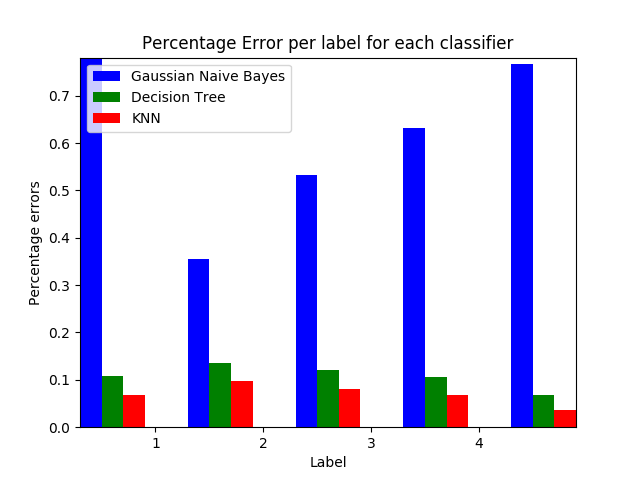
\includegraphics[width=0.7\linewidth]{img/percentage_test_errors_per_label}
	\caption{Percentuale di errore nella predizione per etichetta}
	\label{fig:percentagetesterrorsperlabel}
\end{figure}


\section{Un rimedio ingenuo al rumore}
Un approccio ingenuo per risolvere il problema al rumore potrebbe essere quello di prendere meno dati per etichetta. Il seguente grafico pero' ci mostra che cio' non e' vero

\begin{figure}[H]
	\centering
	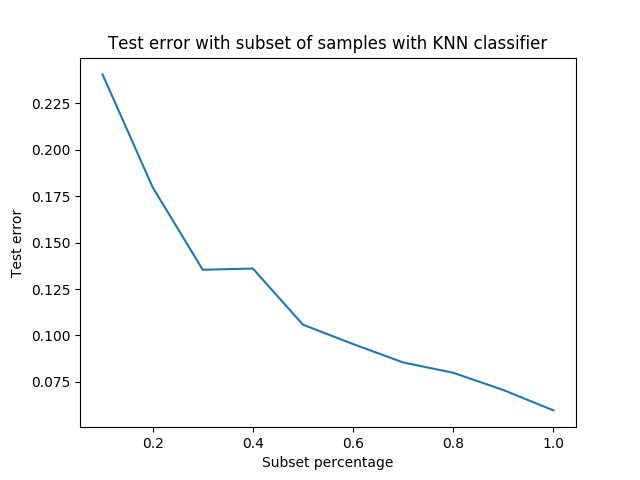
\includegraphics[width=0.7\linewidth]{img/rumor_graph_knn}
	\caption{}
	\label{fig:rumorgraphknn}
\end{figure}


%Ricorda di far vedere falsi positivi e veri negativi nei test